\section{Технологическая часть}

\subsection{Выбор технологических средств}
В качестве языка программирования был выбран Python, поскольку он предоставляет множество необходимых для реализации поставленной задачи библиотек, такие как aiohttp, socket, bencodepy и прочие, а также ввиду имеющего опыта работы с этим языком. 

Была выбрана среда разработки PyCharm, поскольку она бесплатна для студентов и хороша знакома, так как активно использовалась в процессе обучения.

Для создания удобного, интуитивно понятного интерфейса использовался набор библиотек PyQt5. \newline

\subsection{UML диаграмма классов}
На Рисунках \ref{fig300:image}-\ref{fig301:image} приведена UML-диаграмма основных разработанных классов. На диаграмме \ref{fig301:image} приведены все виды сообщений, которыми могут обмениваться участники процесса скачивания.

\newpage

\begin{figure}[h!]
	\begin{center}
		{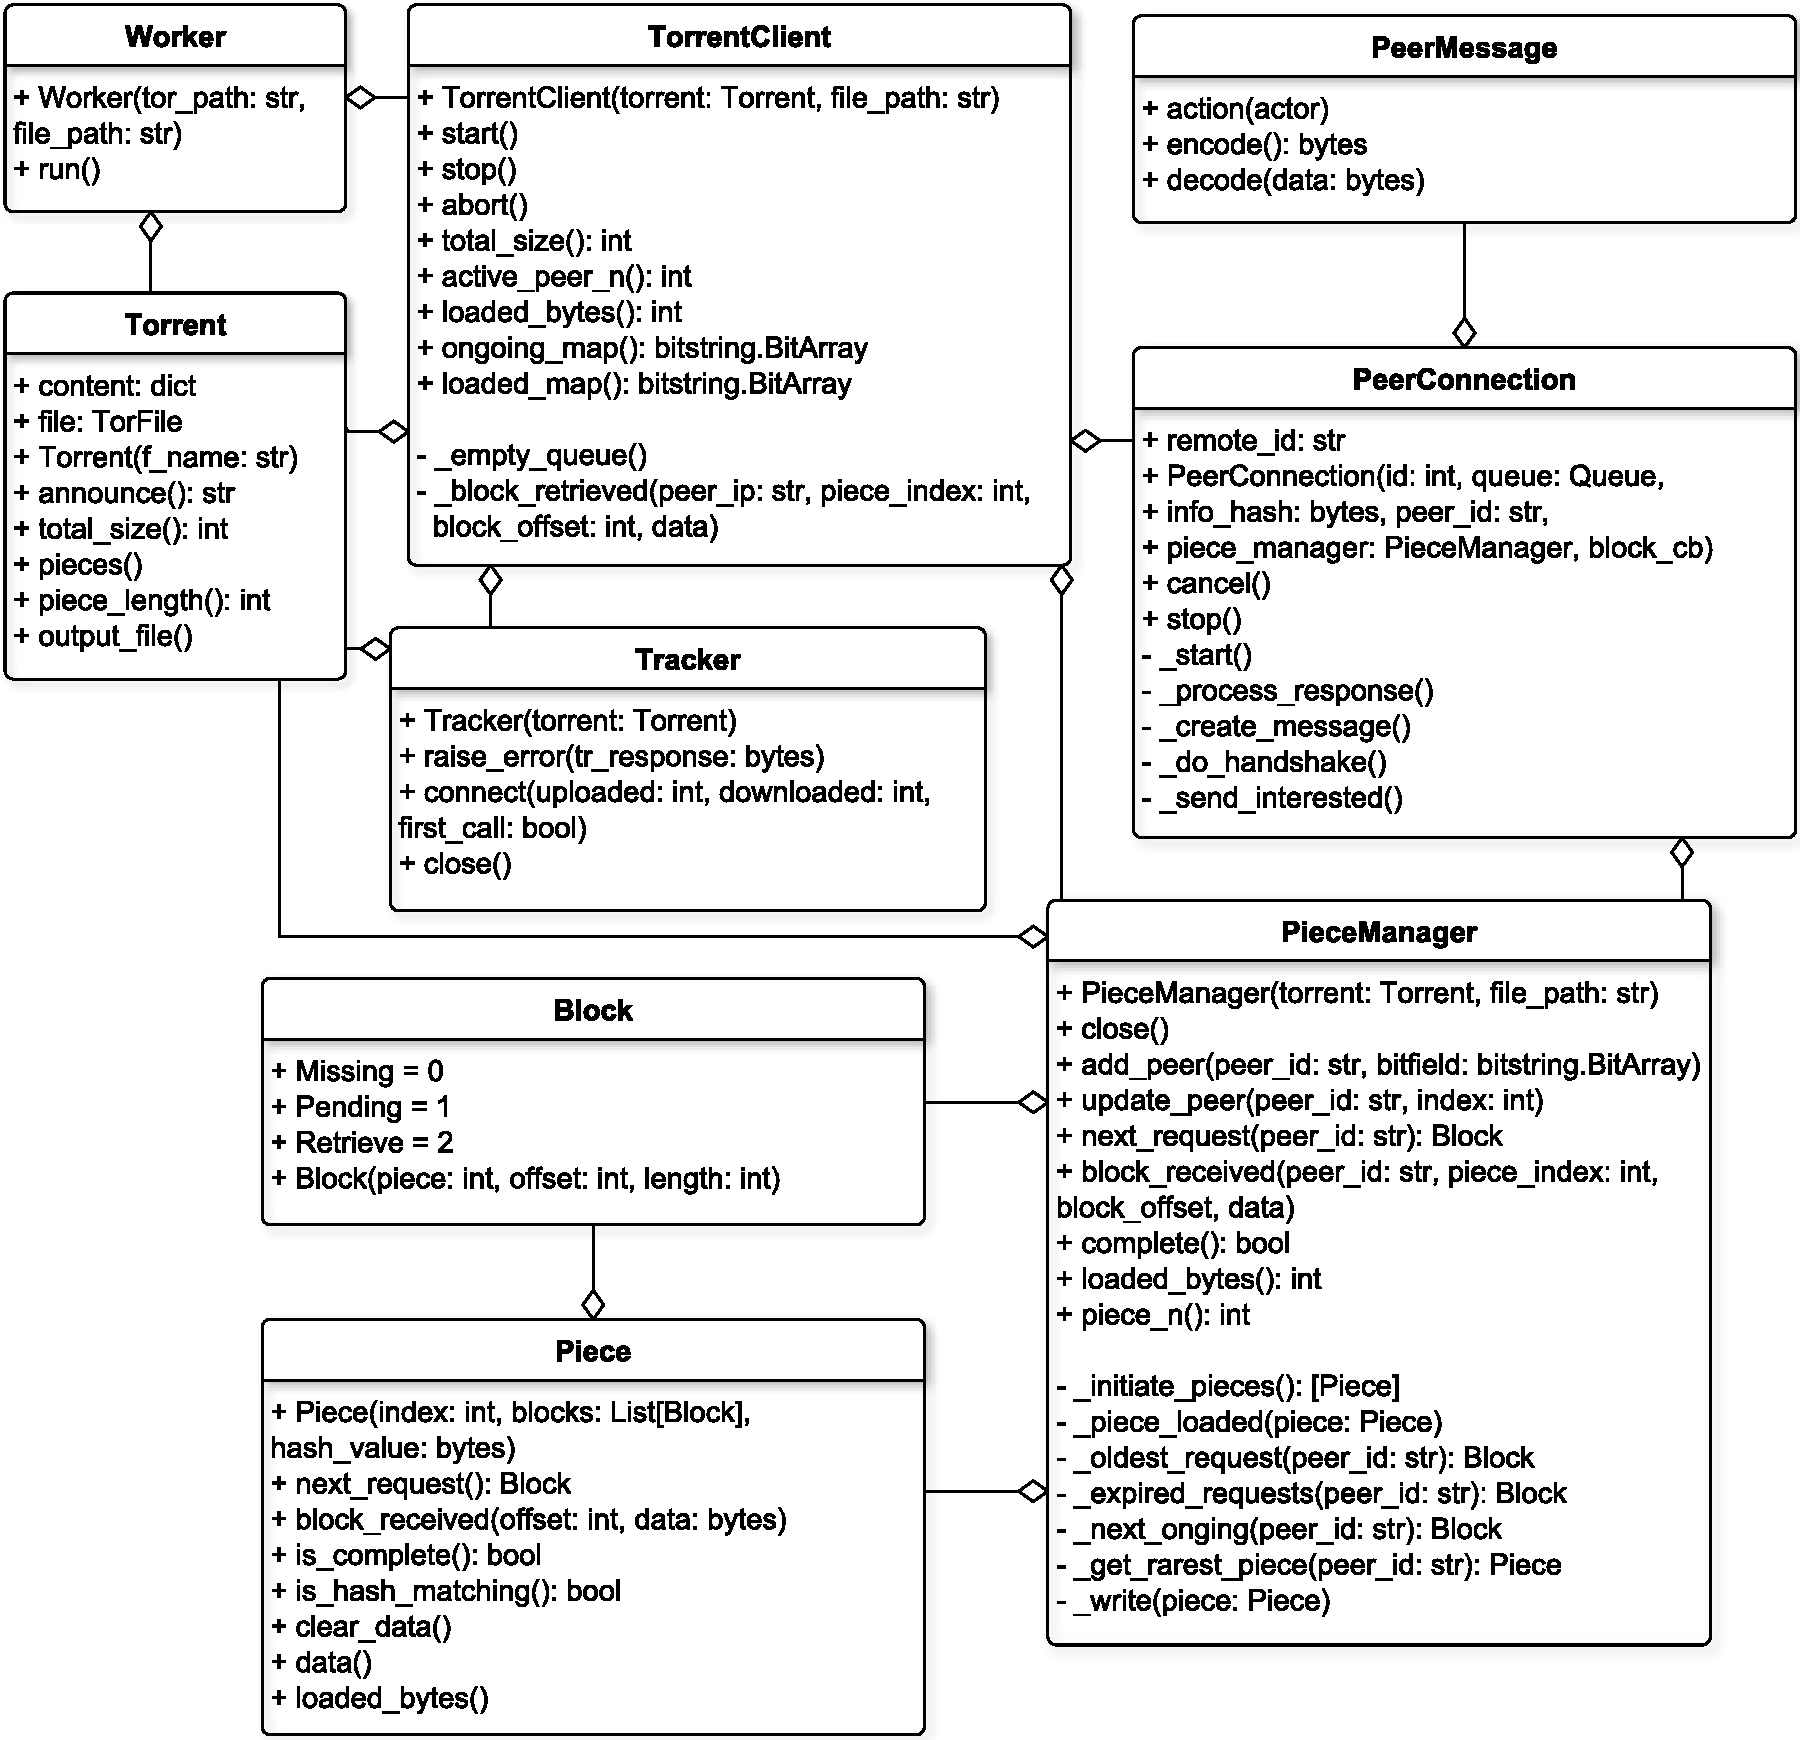
\includegraphics[scale = 0.57]{img/uml.pdf}}
		\caption{UML-диаграмма классов}
		\label{fig300:image}
	\end{center}
\end{figure}

\newpage

\begin{figure}[h!]
	\begin{center}
		{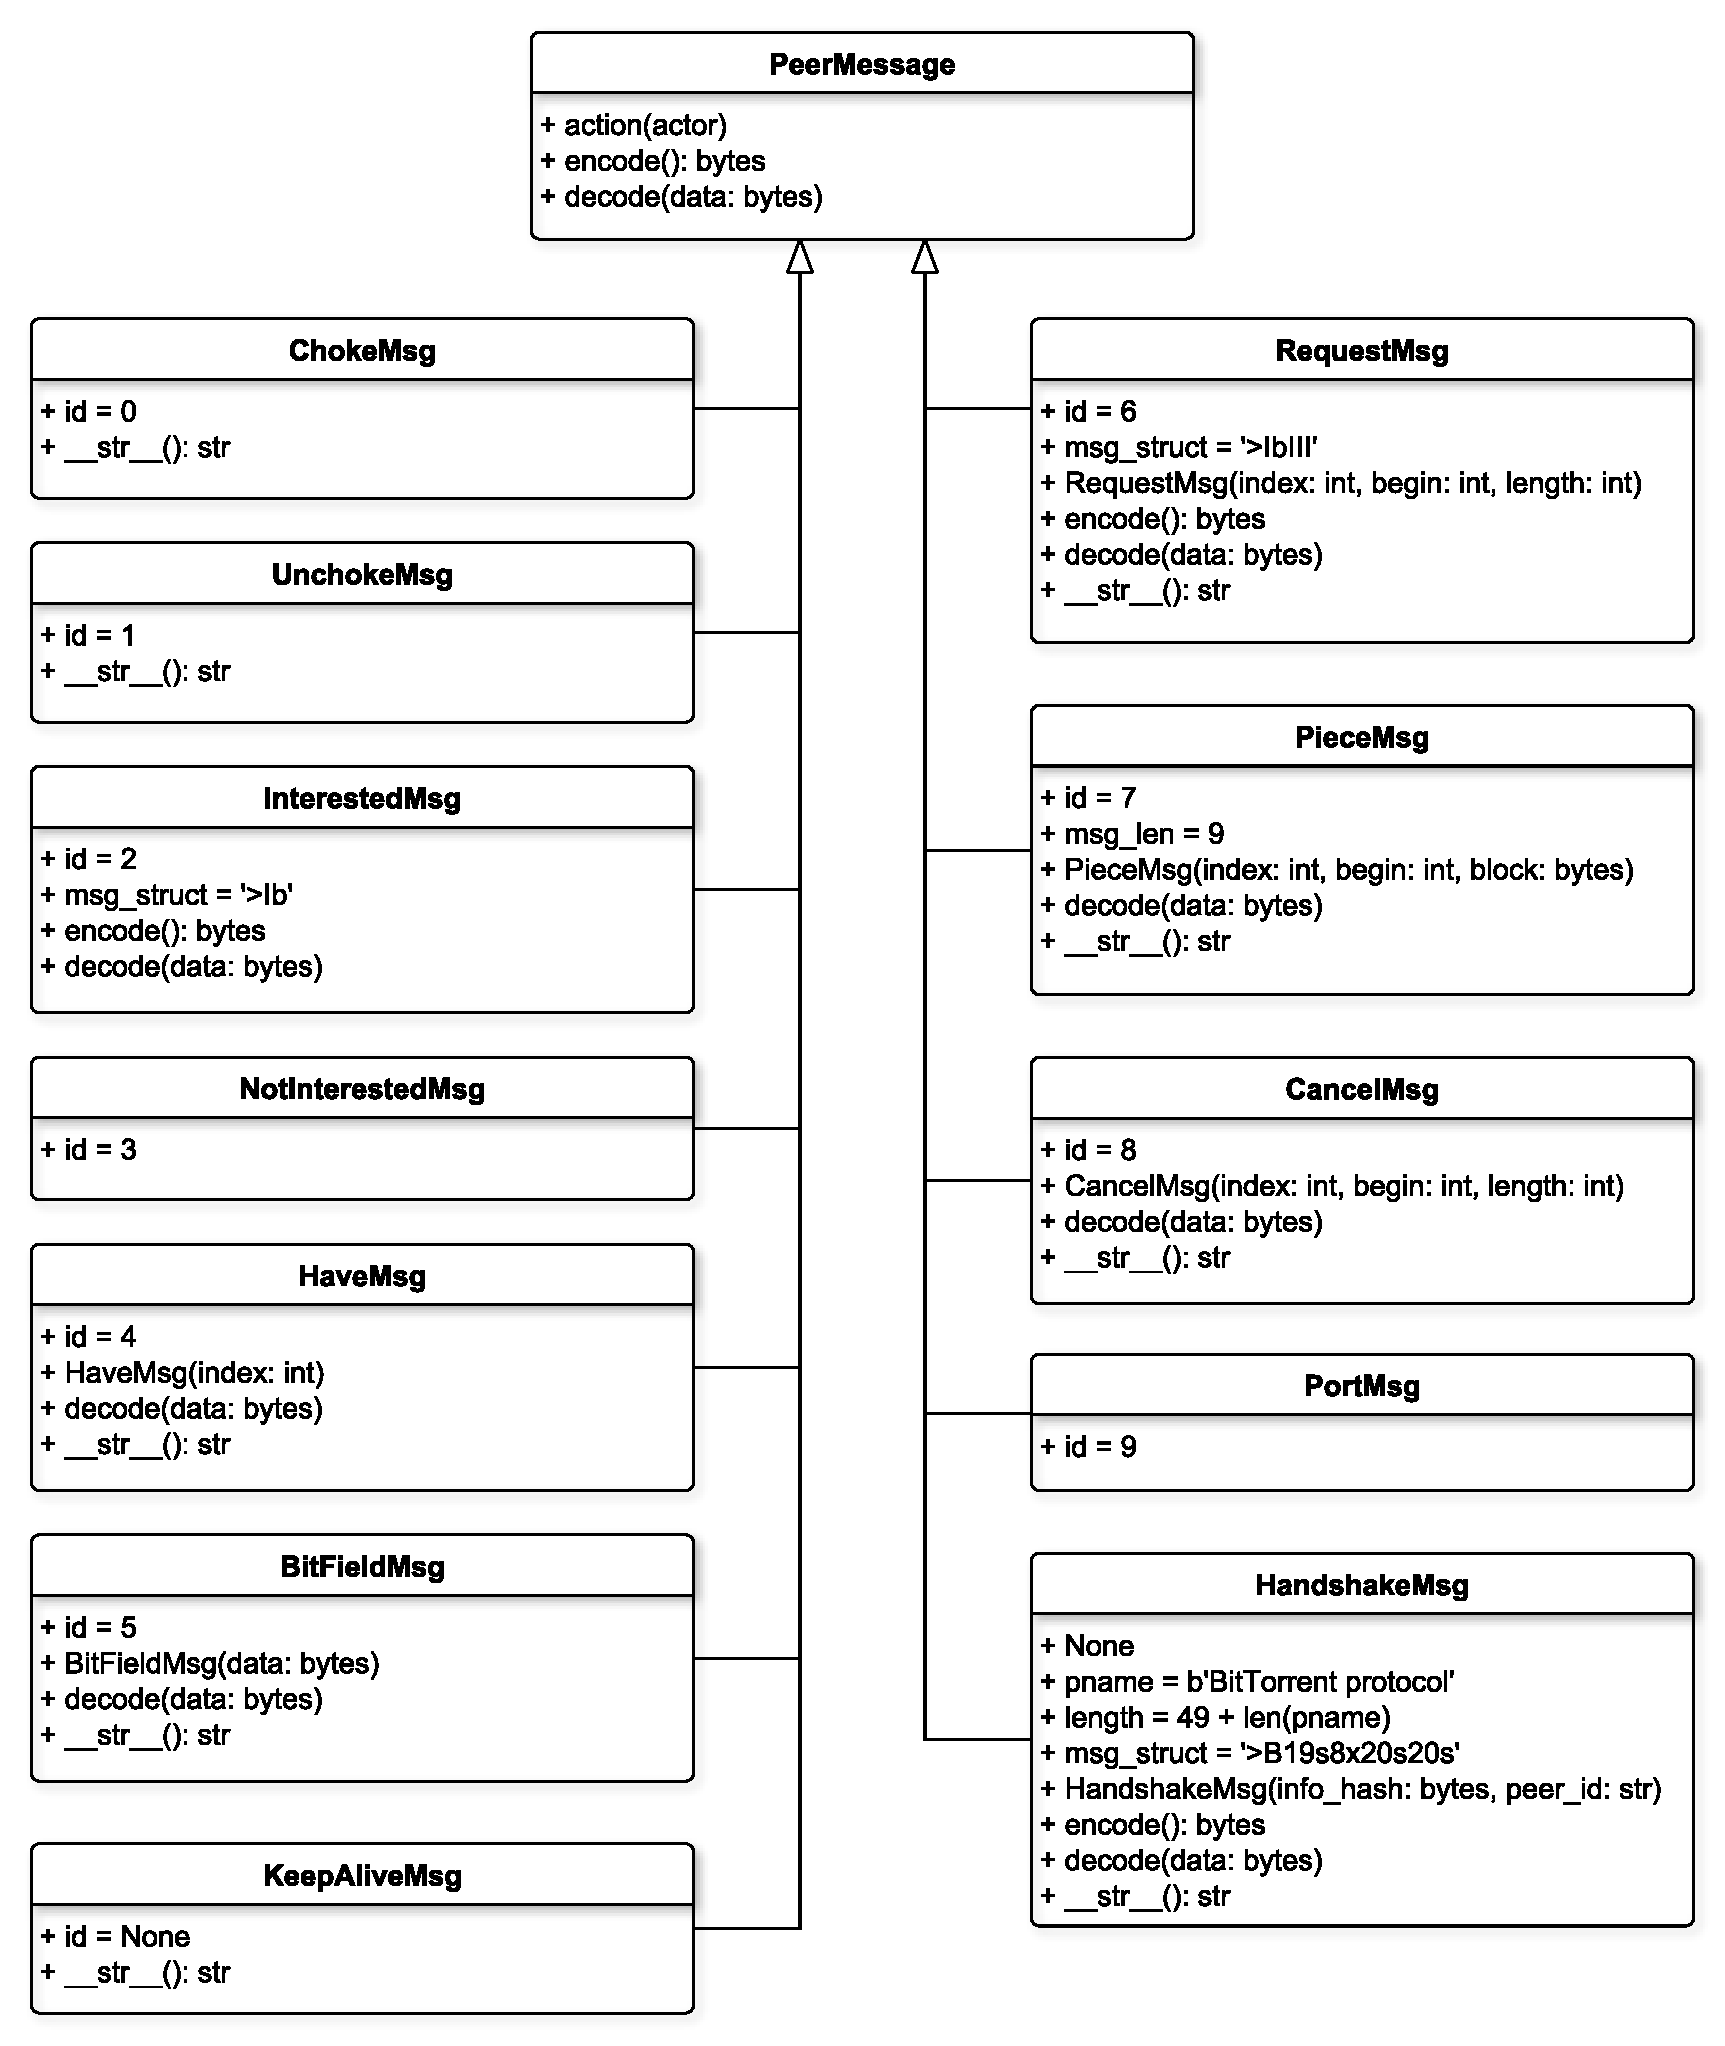
\includegraphics[scale = 0.57]{img/msgs.pdf}}
		\caption{UML-диаграмма классов сообщений}
		\label{fig301:image}
	\end{center}
\end{figure}

\newpage

\subsection{Интерфейс программы}
На Рисунках \ref{fig302:image}-\ref{fig303:image} представлен разработанный графический интерфейс. Для того, чтобы начать процесс скачивания, необходимо сначала указать путь до .torrent файла и выбрать директорию загрузки. Нажатие кнопки <<Старт>> запустит процесс.
\begin{figure}[h]
	\begin{center}
		{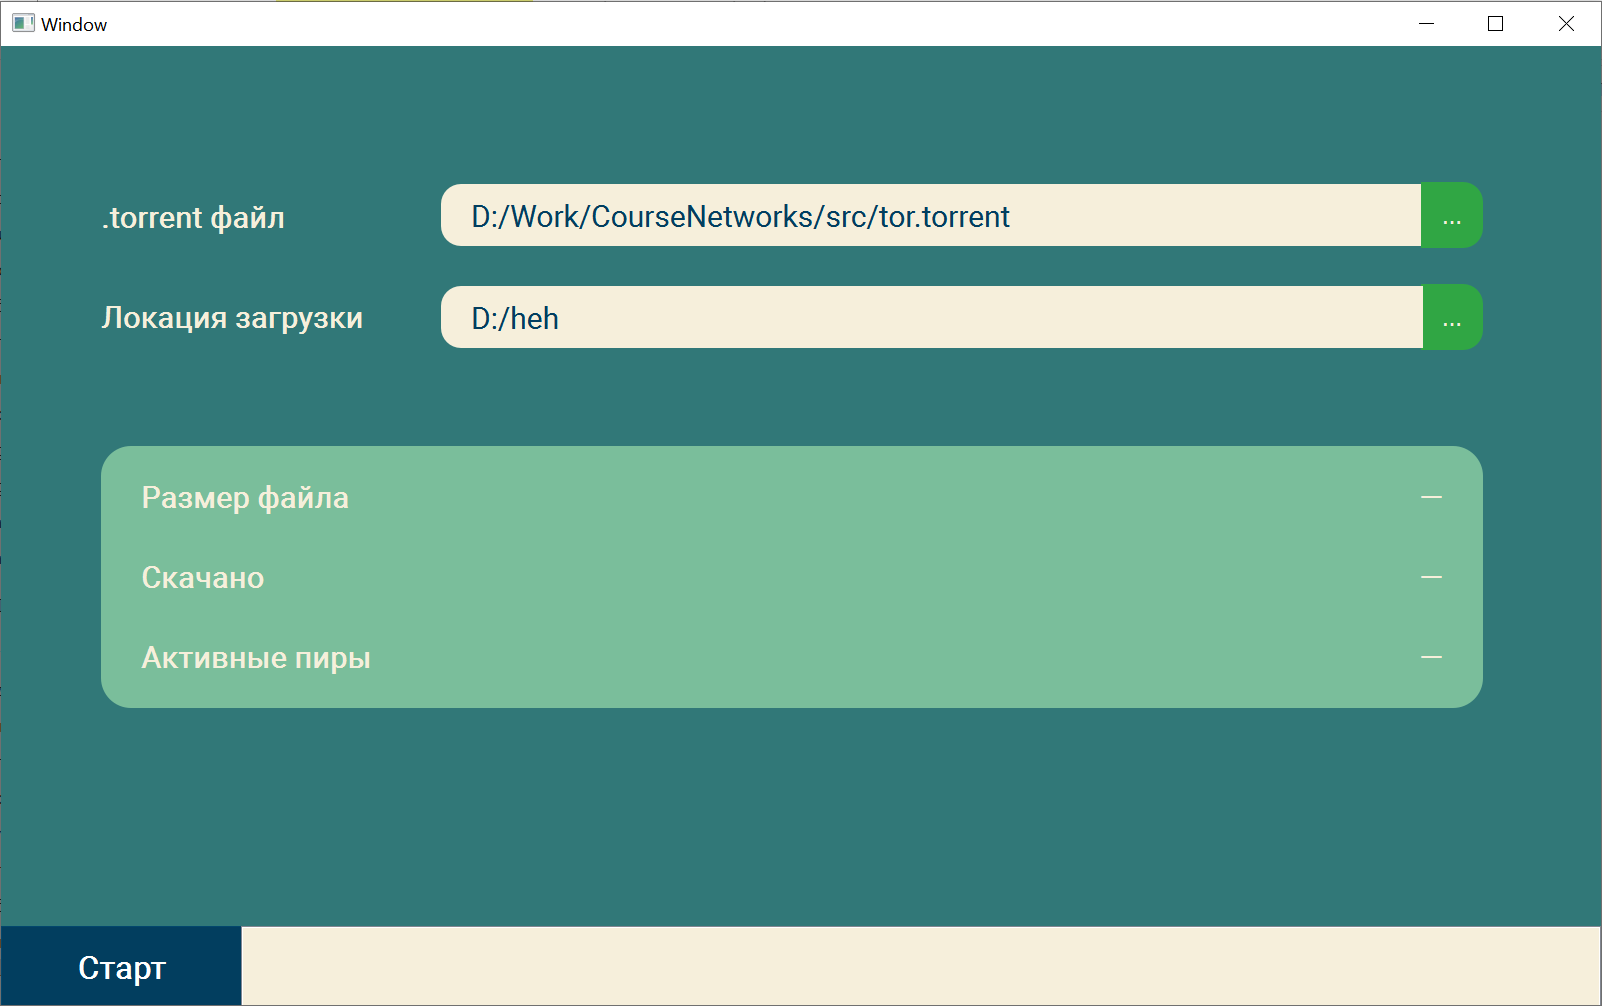
\includegraphics[scale = 0.57]{img/interface_before.png}}
		\caption{Графический интерфейс до начала скачивания}
		\label{fig302:image}
	\end{center}
\end{figure}

В процессе скачивания необходимого файла на экран выводится статистика: размер файла в килобайтах, успешно полученный объём (килобайты) и число активных пиров, с которыми на данный момент происходит взаимодействие.

Для наглядности снизу была добавлена специальная шкала, в которой жёлтым цветом помечаются куски (pieces), находящиеся в процессе скачивания, зелёным -- успешно полученные. Очевидно, когда файл будет полностью скачен, вся полоса будет покрашена в зелёный цвет. \\

\begin{figure}[h]
	\begin{center}
		{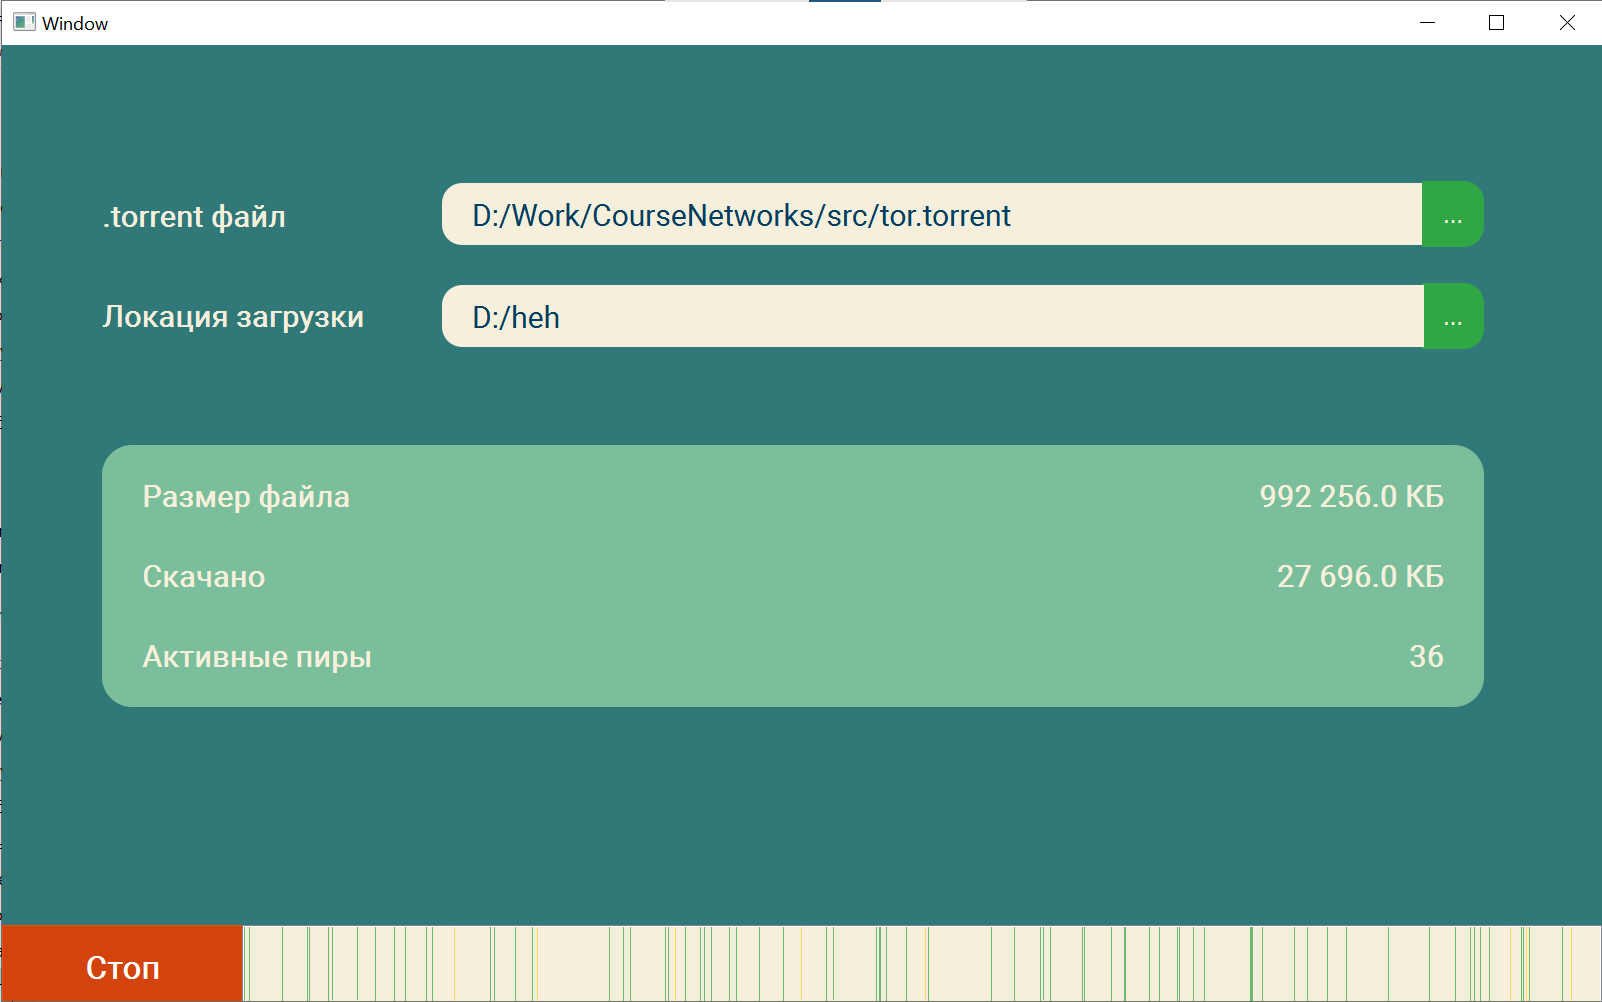
\includegraphics[scale = 0.57]{img/interface_ongoing.png}}
		\caption{Графический интерфейс в процессе скачивания}
		\label{fig303:image}
	\end{center}
\end{figure}

Для того, чтобы прервать операцию, достаточно нажать на кнопку <<Стоп>>.